\chapter{État des lieux démographique}
\paragraph{}Les médias et les politiques nous rabâchent sans cesse que la population vieilli, que le système de pension n’est plus tenable mais qu’en est-il vraiment de la situation en Europe ?  Dans un premier nous allons analyser la démographie actuelle dans l’union Européenne, ainsi que les projections.

\paragraph{}Tout d'abord, quand on parle de vieillissement de la population de quoi parle-t-on ? D’après l’encyclopédie Larousse\citep{larousse}: 
\begin{quotation}
\textit{Le « vieillissement démographique » ou « vieillissement d'une population » désigne une modification progressive de la structure par âge de cette population. L'augmentation de la proportion des personnes âgées (60 ans et plus) s'accompagne d'une diminution, d'abord de la proportion des enfants (moins de 15 ans), puis de la proportion des personnes en âge de travailler (de 15 à 59 ans).}
\end{quotation}

\paragraph{}On retrouve une définition similaire ici\citep{etudiant}.
\begin{quotation}
\textit{Le vieillissement désigne l’augmentation du poids des personnes âgées dans l’ensemble de la population.}
\end{quotation}

\paragraph{}Se doter d’une définition est la première étape mais il faut aussi être capable de mesurer ce vieillissement. Quels en sont les indicateurs ? Jacques Dupâquier \citep[pp.10-11]{dupaquier} en propose sept. 
\begin{enumerate}
  \item \textbf{l’effectif absolu de la population}, il suffit simplement de compter la population plus âgées qu’une limite définie 60, 65 ans. Cette mesure toute seule ne donne aucune indication par rapport au vieillissement de la population si la croissance constaté est proportionelle à la croissance globale de la population.
  \item \textbf{la proportion de la population âgée dans la population totale}. Encore une fois ici il faut définir un seuil, 60 ou 65 ans mais cette mesure est très proche de la définition donné plus haut. 
  \item \textbf{l'âge moyen de la population} et \textbf{l’âge median de la population}. Ces mesures sont très simple et ne nécessitent pas de paramétrage. Une augmentation de cette mesure fait effectivement le constat d’un vieillissement de la population. Mais dans une perspective économique, elle ne donne pas assez d’information. 
  \item \textbf{l’indice de vieillissement}, c’est-à-dire, le nombre de personne âgée sur le nombre de jeune. Il faut ici définir ici deux limites, la limite des jeunes habituellement 15 ans et la limite pour les vieux, habituellement 60 ou 65 ans.
  \item \textbf{l’indice de sénescence}, ici, il faut d’abord définir la limite entre personnes âgées et non âgées et ensuite on définit une seconde limite pour les personnes très âgées par exemple 75 ans et on calcul le rapport personne très âgées / total des personnes âgées. Cette indice ne permet pas de mesurer le vieillissement en tant que tel, mais il permet de le caractérisé.
  \item \textbf{l’indice de dépendance}, cet indice consiste à calculer le rapport entre les personnes dépendantes et les personnes dont elles dépendent. Typiquement le jeune (-15 ans) et les personnes âgées (+65 ans) divisée par la catégorie intermédiaire (15 - 64 ans). Il peut se calculer seulement en tenant compte des personnes âgées. Cette mesure est très intéressante d’un point de vue économique. 
\end{enumerate}
\paragraph{} Sur ces sept mesures, nous en retiendrons principalement deux : la proportion de la population âgée dans la population totale pour mesuré l’ampleur du phénomène et l’indice de dépendance qui permettra de mesurer certain aspect de l’impact du vieillissement. Dans un premier temps nous utiliserons surtout la deuxième. Cependant comme nous l’avons expliciter plus haut, pour pouvoir calculer cet indice, il faut choisir une limite arbitraire entre les personnes âgées et les autres. Dans ce document, nous nous intéressons surtout aux aspects économiques du vieillissement de la population. Il serait donc intéressant de définir la tranche de personne âgées comme les personnes qui ne font plus partie de la population active dû à leur âge. Hélas, avec des régimes de retraite différent dans chaque pays\citep{age_retraite}, et la notion de pré pension, il n’est pas facile de définir une limite bien précise. Nous avons décidé de mettre la limite à 65 ans car il correspond à l’âge de départ à la retraire le plus répandu et surtout parce que les données statistiques sont plus facile à trouver pour cette limite. 

\section{Démographie de l'Europe}
\paragraph{}Maintenant que nous avons clarifier le concept de vieillissement, observons les chiffres de l’Europe. Dans un premier temps, nous avons compiler les données venant de Eurostat\citep{eurostat_pop}, nous avons pris le nombre d’habitants dans 25 pays de l’union européenne, c’est-à-dire tout les pays à l’exception de Malte, Chypre et la Croatie pour lesquels des données manquait. La proportion de la population de ces pays n’est pas important, il n’aurait pas pu influencé beaucoup la tendance globale observée. Nous tirons pouvons donc tirer des conclusion pour toutes l’union européenne malgré le manque de donnée pour ces pays.

\paragraph{}Le graphique \ref{eu_demo} montre l’évolution de la population totale et l’évolution de la population des personnes âgées de plus de 65 ans. On peut observer que la population total est passée de 450 à 500 millions d’habitants entre 1975 et 2013 mais la population de personnes âgées est passé de 55 millions à 91 millions. Elle a presque doublé en un peu moins de 40 ans, alors que la population n’a pas augmenté dans les même proportions. Le graphe \ref{pop_65} montre les choses beaucoup plus clairement. Il montre l’évolution de la proportion de la population âgée de plus de 65 ans. La proportion est passée de 12\% à 18\% en l’espace de 40 ans et surtout de 15,5\% à 18\% en l’espace de 13 ans, on voit que le phénomène s'accélère.  Et cela alors que la proportion de personnes âgées de plus de 65 ans dans le monde n’est que de 12\%\citep{ined}. Il est clair que la population de l’Europe est plus veille que celle du reste du monde et que le phénomène s’accentue d’année en année. 


\begin{figure}[h!]
    \begin{center}
        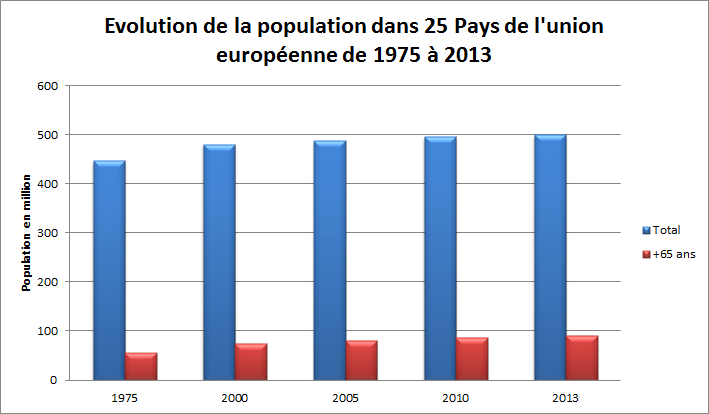
\includegraphics[scale=0.7]{document/pop_eu.png}
        \caption{Évolution de la population dans l'union européenne de 1975 à 2015. Source: Eurostat\citep{eurostat_pop}}
        \label{eu_demo}
    \end{center}
\end{figure}


\begin{figure}[h!]
    \begin{center}
        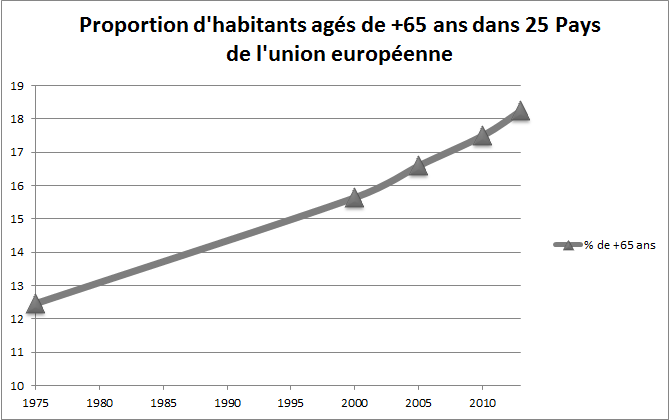
\includegraphics[scale=0.7]{document/pop_65.png}
        \caption{Évolution de la proportion de la population agée de plus de 65 ans dans l'union européenne de 1975 à 2015. Source: Eurostat\citep{eurostat_pop}}
        \label{pop_65}
    \end{center}
\end{figure}


\section{Disparité au sein de l'union européenne}
\paragraph{}Derrière ces chiffres globaux se cachent parfois des réalités parfois très différentes comme nous allons l’observer pour la France et l’Allemagne. Si en 2000, les deux pays on une proportion de 16\% de personnes âgées de plus de 65 ans. Ce n’est plus du tout le cas en 2013 comme le montre le graphe \ref{fr-de_comparaison}. L’Allemagne a maintenant presque 21\% de ce population âgés de plus de 65ans alors que la France est restée plus ou moins stable jusqu’en 2011 et n’atteint pas les 18\% de la moyenne européenne en 2013. La population a continué à croître en France alors qu’elle diminue en Allemagne. Cette différence ne s’explique pas par l’immigration mais par des taux de natalité assez différents: 1,37 en Allemagne et 1,96 en France en 2007.\citep[pp.5]{frde} La moyenne Européenne était de 1,61 dans l’Europe des 28 en 2009. Les différences n’ont pas l’air très importantes mais le graphe \ref{fecondite}\footnote{Ce graphe a été construit en prenant 100 femme pour la première génération et le nombre de femme des génération suivante ce calcule comme suit : $ NBF(X) = \frac{NBF(X-1) * Taux}{2}$} simule l’effet des différents taux de natalité sur la population, montre que pour 100 femmes à la première génération, l’effet cumulé des différents taux de fécondités est exponentiel. Avec un taux de fécondité de 1,38, il ne reste plus que 20 femmes au bout de la 5ème génération alors qu’avec un taux de 1,6 il en reste le double et avec un taux de fécondité supérieur à 2, la population augmente bien entendu.  
 
\begin{figure}[p]
    \begin{center}
        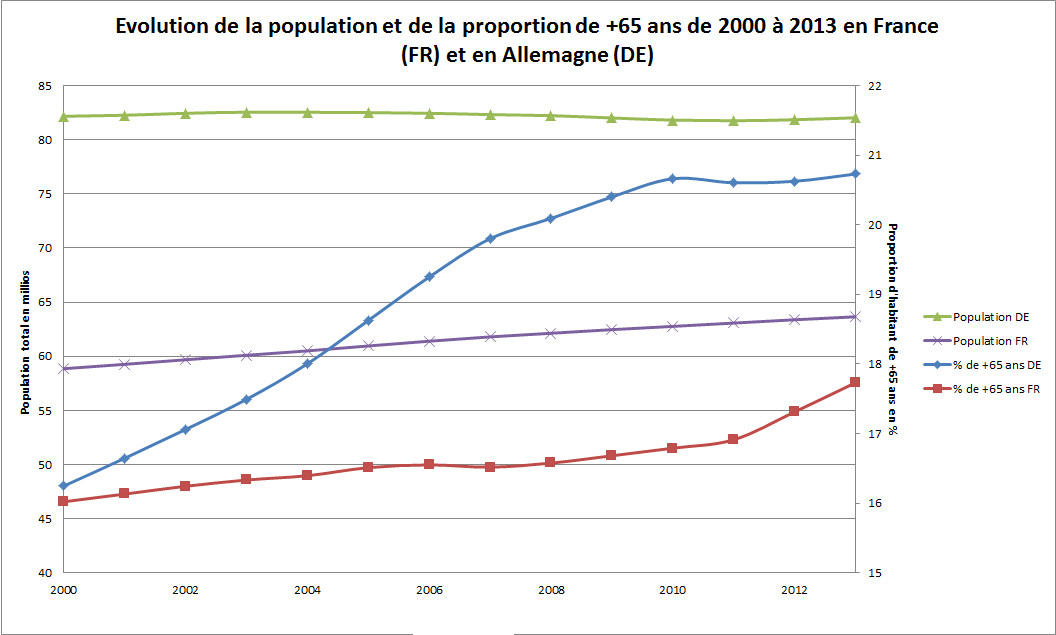
\includegraphics[scale=0.55]{document/fr-de_comparaison.png}
        \caption{Évolution de la population et de la proportion de la population agée de plus de 65 ans en France et en Allemagne de 2000 à 2015. Source: Eurostat\citep{eurostat_pop}}
        \label{fr-de_comparaison}
    \end{center}
\end{figure}

\begin{figure}[p]
    \begin{center}
        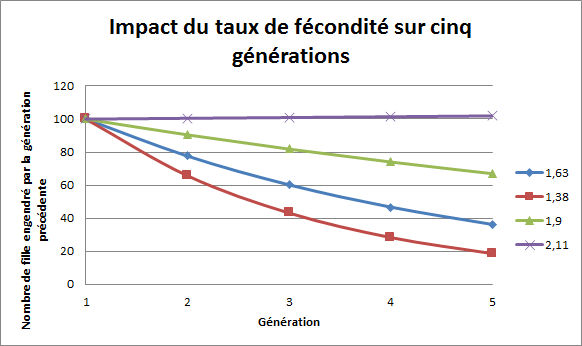
\includegraphics[scale=0.8]{document/fecondite.png}
        \caption{Simuluation de l'évolution du nombre de femme avec différent taux de fécondité constant}
        \label{fecondite}
    \end{center}
\end{figure}

\paragraph{}Quel est le rapport entre le taux de fécondité et le vieillissement de la population ? Nous avons vu que chaque génération va engendré une autre moins nombreuse, mais les anciennes génération continue de vivre un certain temps. Nous avons donc une pyramide des âges inversée qui devient plus petite à la base qu’au sommet et automatiquement la proportion des personnes plus âgées augmente. On peut déjà observé cet effet sur la pyramide des âges de l’Allemagne en 2008. Bien entendu cet effet est atténué par l’immigration. Par contre en France, cet effet n’est pas visible, le bas de la pyramide a tendance à être droite.  En Allemagne, comme en France, on peut observer l’effet du “Baby Boom”\footnote{\textit{Le baby boom ou « pic de la natalité » est une augmentation importante du taux de natalité dans certains pays, juste après la fin de la Seconde Guerre mondiale. Les enfants nés durant cette période sont parfois appelés des « baby boomers » (voir simplement, au Canada, des « boomers »). Cette période s'étend de 1945 jusqu'à 1975.}\citep{baby-boom}} sur les tranches entre 35 et 60 ans qui sont significativement plus importante. On peut observer également que cet effet à duré plus longtemps en France.

\paragraph{}Le cas de l’Allemagne est symptomatique de la plupart des pays européen. Beaucoup de pays présente une courbe similaire à celle de l’Allemagne en 2010 (figure \ref{pyramide-allemagne-france}) avec une base moins resserrée car l’Allemagne est un des pays avec le plus faible taux de natalité. La France, quant à elle, représente plus un exception avec son taux supérieur à 2. C’est donc tout naturellement que la pyramide de l’Europe (Figure \ref{eu-2006}) se retrouve avec une base plus serrée et les tranches des personnes nées pendant le “Baby Boom” plus grande. 

\paragraph{}Après avoir fait le constant sur le passé et le présent, il est intéressant de ce tourner vers l’avenir et de regarder du coté des projections démographique. Les pyramides que nous venons d’observer n’augurent rien de bon. La mise à la retraire des Baby Boomer vient à peine de commencer et ne s’achèvera que dans 25, 30 ans. Toutefois avant cela, il est intérressant de comprendre les causes de ce vieillissement, ce qui nous permettra de mieux comprendre ce que le futur nous réserve. 

\begin{figure}[p]
    \begin{center}
        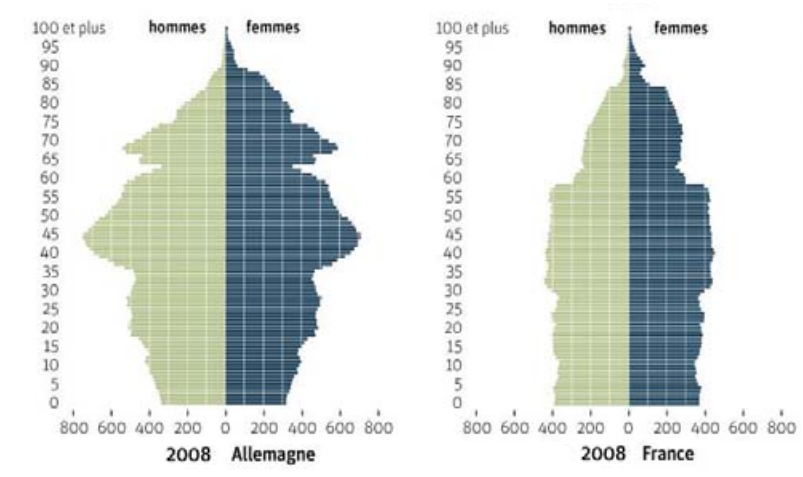
\includegraphics[scale=0.55]{document/pyramide-allemagne-france.png}
        \caption{Pyramide des âges de l'Allemagne à gauche et de la France à droite. Source: Sievert\citep[pp.27]{frde}}
        \label{pyramide-allemagne-france}
    \end{center}
\end{figure}

\begin{figure}[p]
    \begin{center}
        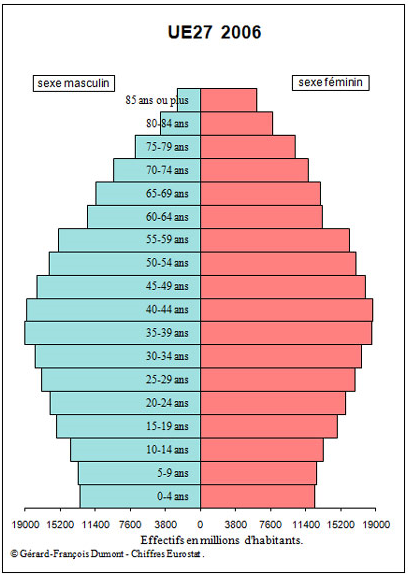
\includegraphics[scale=0.55]{document/eu-2006.png}
        \caption{Pyramide des âges de l'union européenne en 2006 Source: Dumont\citep[pp.3]{pyramide-eu}}
        \label{eu-2006}
    \end{center}
\end{figure}


\section{Facteurs explicatifs du vieillissement démographique}
\paragraph{}Maintenant que nous avons constaté le vieillissement effectifs de la population, il est faut s'interroger sur les causes de celui-ci. L’article de Francois Héran\citep[pp.1]{heran} identifie quatre causes. La première qu’il appel “Vieillissement par le bas”, parce qu’on peut observer son effet par un rétrécissement de la base de la pyramide. Cet effet est dû à une fécondité qui est durablement sous le seuil de remplacement\footnote{\textit{Le seuil de renouvellement (ou de remplacement) des générations, c'est-à-dire le nombre moyen d'enfants par femme nécessaire pour que chaque génération en engendre une suivante de même effectif, est au minimum de 2,05 enfants par femme, soit 205 enfants pour 100 femmes, parce que pour 105 garçons il naît 100 filles. Les seuils réels sont supérieurs à ce minimum en raison de la mortalité entre la naissance et l'âge de procréation.}\citep{renouvellement}
} qui actuellement de 2,07 en Europe. Le graphe \ref{fertilite_eu} montre le taux de fertilité de ces 15 dernières années dans l’Europe des 28. La tendance est clair, le taux de fertilité est bien en dessous du taux de remplacement et il n’est pas près de remonté. Du fait de la baisse des jeunes, la proportion de personnes âgée augmente de facto.  

\paragraph{}Le second effet est ce qu’appel Héran\citep[pp.1]{heran}, le “vieillisement par le haut”, c’est-à-dire, l’ajout d’étage supplémentaire en haut de la pyramide des âges dû à l’augmentation de l’espérance de vie.  Les personnes de plus de 65 ans au lieu de mourir, vieillissent. Cette progression de l’espérance de vie a dépassé les projections. Chaque année, un gain de deux à trois mois est observé. Ce facteur est vu comme inévitable car personne ne peut mettre en place une politique qui vise à réduire la progression de l’espérance de vie.

\paragraph{}Le troisième facteur est la suite de conséquences des fortes variations de la natalité dans le passé\citep[pp.2]{heran} : Le Baby Boom et puis un retour à la “normal”. Ces trente années de fertilités exceptionnelles ont eu comme effet premier de rajeunir la population, ensuite de grossir les rangs de la population active pendant des dizaines d’année, mais maintenant, il vient participer à l’accélération du vieillissement pour finalement faire monter le taux de mortalité. Si on observe l’évolution d’une pyramide des âges dans un pays comme la Belgique on peut voir clairement une vague se formé à partir des années 50 et se déplacer et être actuellement autour des 55 ans\citep{pyramide-be}. Ce facteur est denouveau inévitable car aucune politique démographique ne peut l’influencer, c’est une conséquence des politique passé.

\paragraph{}Le dernier facteur\citep[pp.3]{heran}, plus anecdotique est l’émigration sélective des jeunes. Ce phénomène peut s’observer en Albanie par exemple.

\begin{figure}[h!]
    \begin{center}
        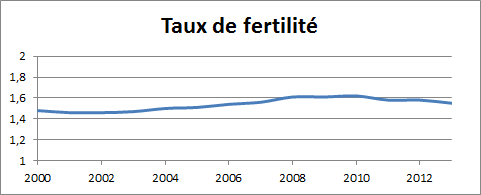
\includegraphics[scale=1]{document/fertilite_eu.png}
        \caption{Variation du taux de fertilité pour l'Europe des 28 de 2000 à 2013.  Source: Eurostat\citep{eurostat_fecondite}}
        \label{fertilite_eu}
    \end{center}
\end{figure}

\section{Projection démographique}
\paragraph{}Deux projections sont facilement disponible pour l’Europe, celle de l’ONU\citep{onu} et celle d’Eurostat\citep{eurostat_europop13}. Les données d’Eurostat concerne plus spécifiquement l’union européenne, le sujet de notre étude. Nous allons donc surtout nous focaliser sur celle-ci.  

\subsection{Les hypothèses des projections d’Eurostat}
\paragraph{}Les projections sont construites sur base d’une année de référence, ici 2013 pour EUROPOP2013\citep{eurostat_europop13}, selon la formule suivante:
$$ Pop_{1.1.n+1} = Pop_{1.1.n} + naissances_{n} - deces_{n} + solde migratoire_{n} $$ \citep[pp.3]{INSEE}
où $Pop_{1.1.n}$ est la population au premier janvier de l'année n et $Pop_{1.1.n+1}$ est la population au premier janvier de l'année suivante. Cette formule assez simple cache beaucoup de complexité, les naissances sont basées sur le nombre de femme à l’année n, sur leur âges et sur le taux de fécondité. Les décès sont basés sur un quotiant de mortalité lui-même basée différent pour chaque l’âge et dépendant de l’espérance de vie, à cela il faut ajouter la mortalité des nouveau-nés\citep[pp.4]{INSEE}. Et bien sur le solde migratoire est basée sur l’immigration et l’émigration à l’intérieur du territoire qu’on étudie. Le rapport “The 2015 Ageing Report” décrit en détails toutes les hypothèses prisent sur ces paramètres\citep[pp.8-14]{ageing_methodo}. Dans les grandes lignes, la projection EUROPOP2013 utilise une approche convergeante, touts les paramètres converge et se stabilise sur une très longue période de temps. Une point de convergence éloigné permet de tenir compte des tendances actuelles mais aussi de partir de l’hypothèse d’une convergence des paramètres sur le long terme. La projection du taux de fertilité est en hausse et convergerait vers 1.76 en 2060\citep[pp.9]{ageing_methodo}. L’espérance de vie va encore augmenter de 7,2 ans pour les hommes (84,7 and en 2060) et des 6 ans pour les femmes jusqu’en 2060 (89,1 ans en 2060)\citep[pp.11]{ageing_methodo}. Le taux de migration est certainement la donnée la plus variable, la projection estime à 55 million le solde migratoire cumulé sur les années de la projection\citep[pp.14]{ageing_methodo}. Nous ne détaillerons pas ici touts les détails des hypothèses ni les calculs qu’elles impliquent car nous serions bien au delà du cadre de ce document. 

\paragraph{}Eurostat fournis cinq scénarios, un scénario principale, un scénario sans migration, une variante de migration basse (48 millions de solde migratoire sur la période jusqu’en 2060)  un scénario avec une espérance de vie haute (en 2060, 86,1 ans pour les hommes et 90,6 ans pour les femmes en 2060) et une hypothèse de fécondité basse (qui converge vers 1,39 en 2060). La table \ref{projection_scenario} présente les résultats de chaque scénario pour 2060 et 2080.

\begin{table}
  \caption{Projection de la population total dans l'Europe des 28 selon les différents scénario d'Eurostat EUROPOP13 source: Eurostat\citep{eurostat_europop13}}
  \label{projection_scenario}

  \begin{center}
    \begin{tabular}{lcc}
       & Population en 2060 & Population en 2080\\
      Scénario principale & 522.945.539 & 520.035.469\\
      Sans migration & 442.752.273 & 399.215.880 \\
      Migration basse & 515.880.322 & 506.906.909 \\
      Espérance de vie haute & 528.301.525 & 533.900.985 \\
      Fécondité basse & 516.144.576 & 497.707.180 \\
    \end{tabular}
  \end{center}
\end{table}

\paragraph{}Mis à part dans le scénario d’une espérance de vie haute, la population entre 2060 et 2080 diminue. Le scénario sans migration est le plus distant du scénario principale et amène une diminution de 43 millions d’habitant en 20 ans. C’est celui qui fait l’hypothèse la plus extrême, il permet de mettre en avant le rôle majeur de l’immigration dans le maintien de l’Europe.


\subsection{Analyse du scénario principale des projections Eurostat}
\paragraph{}Regardons maintenant plus en détails le scénario principale. Nous allons reprendre les même indicateur que dans les section précédentes pour quantifié le vieillissement de la population. 

\paragraph{}Le graphe \ref{proj_pop} montre l’évolution de la population jusqu’en 2080 ainsi que l’évolution de l’âge moyen de la population. La population augmente jusqu’en 2050 et l’âge moyen de la population jusqu’en 2040. On peut observer une nette corrélation entre la population et l’âge moyen de la population, ce qui veut dire que l’augmentation de la population est dû à l’ajout d’étage à la pyramide des âges. En 2040 commence le processus de mortalité des personnes nées pendant le baby boom pour s’achever en 2070. Ce n’est qu’en 2070 que l’union européenne cessera de subir les conséquences du taux de fertilité pendant le baby boom. 


\begin{figure}[h!]
    \begin{center}
        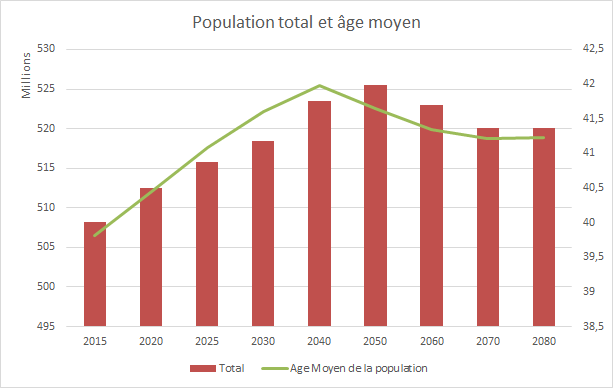
\includegraphics[scale=0.7]{document/proj_pop.png}
        \caption{Projection de la population total et de l'âge moyen de cette population de 2015 à 2080 dans l'Europe des 28. Source: Eurostat\citep{eurostat_europop13}}
        \label{proj_pop}
    \end{center}
\end{figure}

\paragraph{}Le graphe \ref{proj_prop}  présente l’évolution de la proportion de personnes âgées, la courbe suit la tendance observée dans le graphe précédent. La proportion passera de 15\% à 20\% en 2040 pour se stabiliser en 2070 autour de 18\%. Ce graphe montre que si le vieillissement de la population est déjà un problème maintenant il sera plus important de 33\% en 2040. Ce graphe nous montre qu’il ne faudra pas seulement trouver des solutions à court termes mais surtout à long terme.

\begin{figure}[h!]
    \begin{center}
        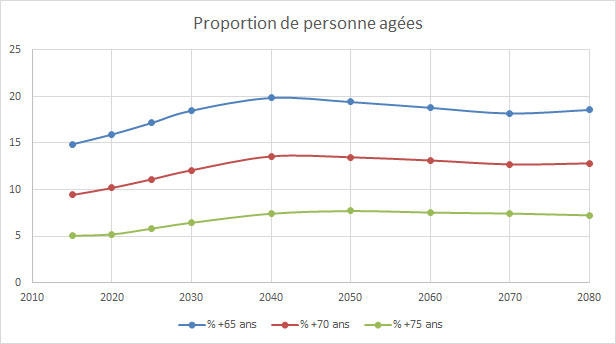
\includegraphics[scale=0.7]{document/proj_prop.png}
        \caption{Projection de l'évolution de la proportion de personnes agées dans la population dans l'Europe des 28 de 2015 à 2080. Source: Eurostat\citep{eurostat_europop13}}
        \label{proj_prop}
    \end{center}
\end{figure}

\paragraph{}Le  graphe \ref{dependance} permet de prendre pleinement la mesure du problème. Il mesure le degré de dépendance, entre d’autre terme le nombre de personne qu’une personne active aura à charge. Bien entendu ce graphe ne tient pas compte des personnes non actives car au chômage, malade ou handicapée.  Le degré de dépendance est de 60\% en 2050 dû en plus grande partie par les personnes âgées\footnote{ Elles pèsent pour 56\% dans l’indice : 34/60}. La courbe de dépendance total est presque parfait corrélée sur la courbe de dépendance total car le nombre d’enfant âgés de moins de 15 reste stable. 



\begin{figure}[h!]
    \begin{center}
        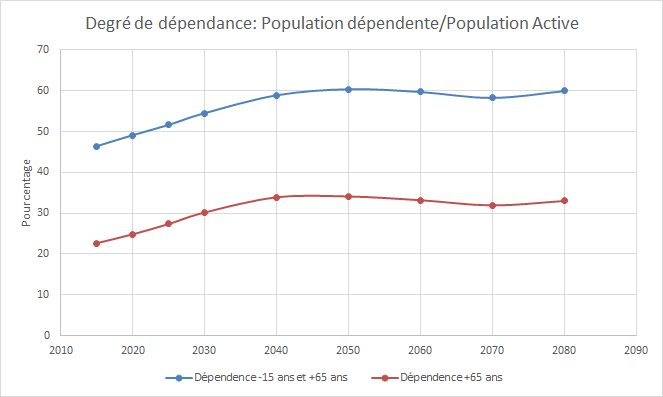
\includegraphics[scale=0.6]{document/dependance.png}
        \caption{Projection de l'évolution du degré de dépendance dans la population dans l'Europe des 28 de 2015 à 2080. Source: Eurostat\citep{eurostat_europop13}}
        \label{dependance}
    \end{center}
\end{figure}

%TODO
\paragraph{}Dans le prochain chapitre nous allons analyser les conséquences économique et social de ce vieillissement durable pour l’union européenne.
